\documentclass{article}
\usepackage[UTF8, heading = false, scheme = plain]{ctex}

\usepackage{geometry}
\geometry{b5paper,left=2cm,right=2cm,top=2cm,bottom=2cm}

\usepackage{color}
\usepackage{amsfonts}
\usepackage{amsmath}

\linespread{1.5}

\usepackage[colorlinks,
            linkcolor=red,
            anchorcolor=blue,
            citecolor=green
            ]{hyperref}

\usepackage{listings}
\usepackage{fontspec}
\usepackage{graphicx}
\usepackage{algorithmic}
\newfontfamily\monaco{Monaco}
\definecolor{dkgreen}{rgb}{0,0.6,0}
\definecolor{gray}{rgb}{0.5,0.5,0.5}
\definecolor{mauve}{rgb}{0.58,0,0.82}
\lstset{ %
  basicstyle=\footnotesize\monaco,       % the size of the fonts that are used for the code
  numbers=left,                   % where to put the line-numbers
  numberstyle=\footnotesize\monaco\color{gray},  % the style that is used for the line-numbers
  numbersep=5pt
  stepnumber=1,                   % the step between two line-numbers. If it's 1, each line
                                  % will be numbered
  numbersep=5pt,                  % how far the line-numbers are from the code
  backgroundcolor=\color{white},      % choose the background color. You must add \usepackage{color}
  showspaces=false,               % show spaces adding particular underscores
  showstringspaces=false,         % underline spaces within strings
  showtabs=false,                 % show tabs within strings adding particular underscores
  frame=lines,                   % adds a frame around the code
  rulecolor=\color{black},        % if not set, the frame-color may be changed on line-breaks within not-black text (e.g. commens (green here))
  tabsize=4,                      % sets default tabsize to 2 spaces
  captionpos=t,                   % sets the caption-position to bottom
  breaklines=true,                % sets automatic line breaking
  breakatwhitespace=false,        % sets if automatic breaks should only happen at whitespace
  title=\lstname,                   % show the filename of files included with \lstinputlisting;
                                  % also try caption instead of title
  keywordstyle=\color{blue},          % keyword style
  commentstyle=\color{dkgreen},       % comment style
  stringstyle=\color{mauve},         % string literal style
  escapeinside={\%*}{*)},            % if you want to add LaTeX within your code
  morekeywords={*,...}               % if you want to add more keywords to the set
}

\usepackage{amssymb} 
\usepackage{amsmath}
\usepackage[ruled,vlined]{algorithm2e}

\setlength{\parindent}{2em}

\renewcommand{\G}{\mathbb{G}}
\newcommand{\Z}{\mathbb{Z}}
\newcommand{\Q}{\mathbb{Q}}
\newcommand{\F}{\mathbb{F}}

\newcommand{\Sbox}{\textsf{Sbox}}
\newcommand{\code}[1]{\lstinline!#1!}

\newcommand{\CKDpriv}{\textsf{CKDpriv}}
\newcommand{\CKDpub}{\textsf{CKDpub}}

%%%%%%%处理下划线:_%%%%%%%%%
\usepackage{underscore}
%%%%%%%处理下划线:_%%%%%%%%%

\setlength{\parindent}{2.1em}

%%%设置页眉和页码格式
\usepackage{fancyhdr}
\newcommand{\makeheadrule}{%
\rule[0.85\baselineskip]{\headwidth}{0.5pt}\vskip-.8\baselineskip}%1.5 0.4->0.5
\makeatletter
\renewcommand{\headrule}{%
{\if@fancyplain\let\headrulewidth\plainheadrulewidth\fi
\makeheadrule}}
\makeatother
\pagestyle{fancy}
\fancyhf{}
\fancyhead[r]{\textit{Crypto In Action}}
\fancyfoot[C]{--{~\thepage~}--}
%%%设置页眉和页码格式结束

\usepackage{color}
\newcommand{\red}{\textcolor{red}}
\newcommand{\blue}{\textcolor{blue}}

\begin{document}

\title{Introducing Paillier Encryption Scheme}
\author{longcpp \\ \small{longcpp9@gmail.com}}

\maketitle

Pascal Paillier在其1999年的论文
``Public-Key Cryptosystems Based on Composite Degree Residuosity Classes''
中引入了Paillier公钥加密机制, 其安全性由合成剩余类(Composite Residuosity Class)
相关的困难问题保证. Paillier的特殊之处是在概率加密的基础之上保留了加法同态的特性.
这一特性被广泛应用于构造各类密码协议, 例如近年来提出应用于数字货币领域的
的两方ECDSA签名协议和多方阈值ECDSA签名协议.

\section{Paillier公钥加密机制}

与其他公钥加密机制一样, Paillier公钥加密机制也由密钥生成(Key Generation)
加密(Encryption)和解密(Decryption)三个算法组成.
三个算法的详细计算过程在图~\ref{fig-paillier}~中展示, 
图~\ref{fig-paillier}~截取自Sigrun Goluch的毕业论文
``The development of homomorphic cryptography''. 
为了理解图~\ref{fig-paillier}~中展示的过程,需要先介绍\textbf{Carmichael函数}的概念.

\subsection{Paillier公钥加密算法}

对于正整数$n$, \textbf{Carmichael函数$\lambda(n)$}表示满足下面要求的最小的正整数$t$:
$$
x^t = 1 ~\textsf{mod}~ n, ~\text{其中}~ x \in \Z ~\text{并且}~ \textsf{gcd}(x, n) = 1.
$$
对于素数$p$, 根据费马小定理可知$\lambda(p) = \varphi(p) = p-1$, 其中$\varphi$表示欧拉函数.
根据代数基本定理可以对任意整数$n$做唯一分解,记为$n = p_1^{a_1}p_2^{a_2}\cdots p_k^{a_k}$,
其中$p_1, p_2, \cdots, p_k$为互不相同的素数. 
R. D. Carmichael在1912年给出了求解$\lambda(n)$的计算公式($\textsf{lcm}$表示最小公倍数): 
\begin{equation*}
\lambda(n) = \textsf{lcm}
\left(
\lambda\left(p_1^{a_1}\right), \lambda\left(p_2^{a_2}\right), \cdots, \lambda\left(p_k^{a_k}\right)
\right),
\lambda(p_i^{a_i}) = 
\left\{
\begin{array}{l}
2^{a_i - 2}, ~\text{for}~ p_i = 2, a_i > 2\\
(p_i - 1)p_i^{a_i - 1}, ~\text{otherwise}~\\
\end{array}
\right.
\end{equation*}
Paillier公钥加密机制中仅关心$n = pq$且$p, q$为大素数的情形, 
根据上式有$\lambda(n)=\textsf{lcm}(p-1, q-1)$, 并且
$\lambda(n^2) = \textsf{lcm}(p(p-1), q(q-1)) = n\cdot\textsf{lcm}(p-1, q-1) = n\lambda(n)$.
则对任意的$x\in \Z_{n^2}^*$, 都有$$x^{n\lambda(n)} = 1 ~\textsf{mod}~ n^2.$$
由于对任意的$x\in \Z_{n^2}^*, ~\textsf{gcd}(x, n^2) = 1$都有$\textsf{gcd}(x, n) = 1$, 
则对于任意的$x \in \Z_{n^2}^*$, 都有$$x^{\lambda(n)} = 1 ~\textsf{mod}~ n.$$

\begin{figure}[h]
\centering
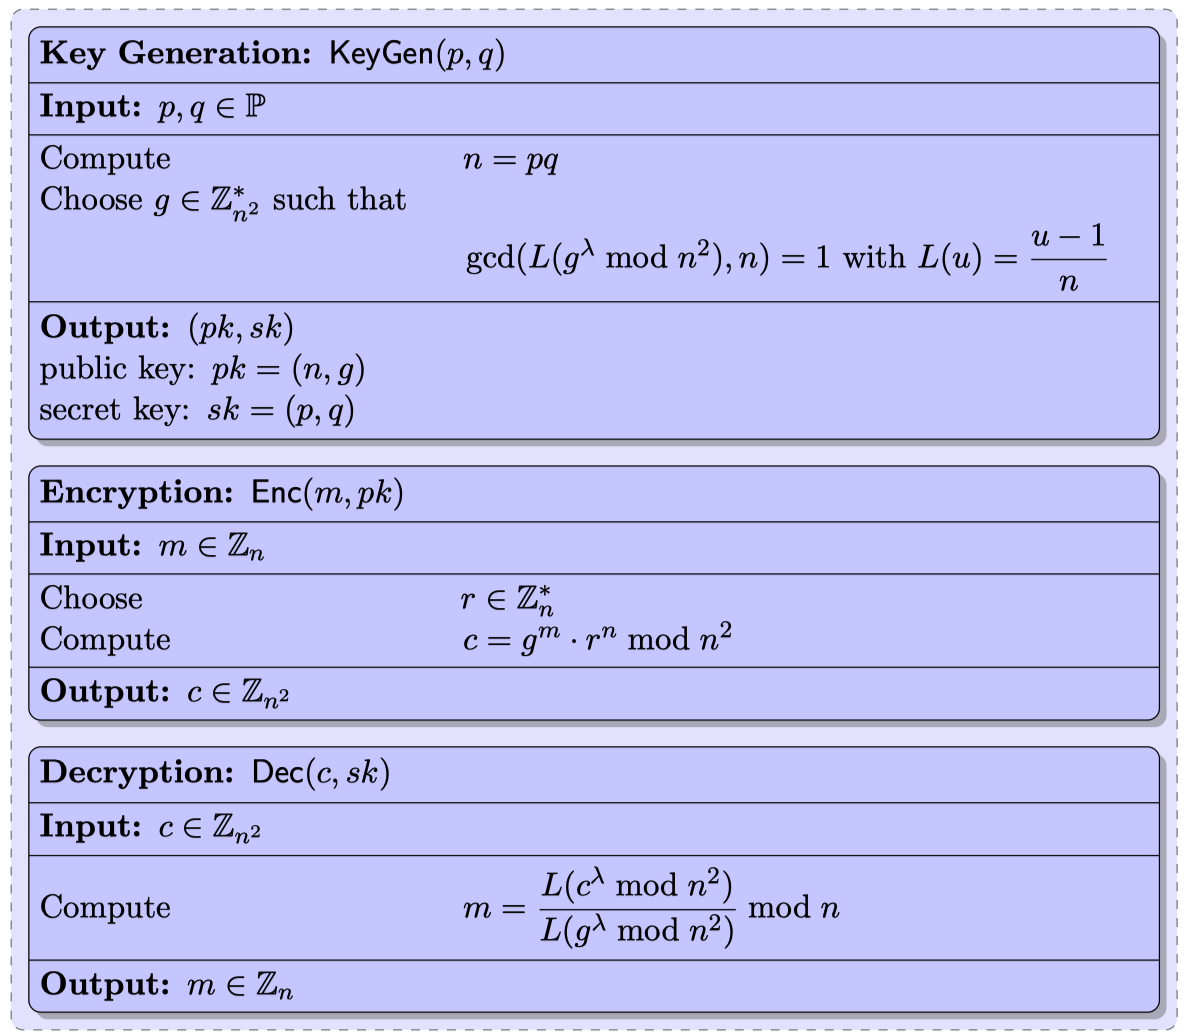
\includegraphics[width=\textwidth]{paillier.png}
\caption{Paillier公钥加密机制}\label{fig-paillier}
\end{figure}

密钥生成算法$\textsf{KeyGen}$的输入为两个大素数$p$, $q$,
而$g$则是从$\Z_{n^2}^*$中选取的满足
$\textsf{gcd}\left(L\left(g^\lambda \mod n^2\right), n\right) = 1$
的元素, 其中的映射$L: \Z_{n^2}^* \rightarrow \Z_n$定义为$L(u) = \blue{\frac{u-1}{n}}$.
值得注意的是,与通常的密码学构造书写规范不同的是,
映射$L$的定义中$\blue{\frac{u-1}{n}}$的含义是,计算$(u-1)$除以$n$的商,
而非在$\Z_{n^2}^*$中计算$(u-1)$乘以$n$的逆. 
Paillier机制的构造能够保证$\blue{\frac{u-1}{n}}$总是能够整除,后续会介绍.
映射$L$输入中的$\lambda$即为之前介绍的Carmichael函数$\lambda(n)$.
关于$g$的约束条件$\textsf{gcd}\left(L\left(g^\lambda \mod n^2\right), n\right) = 1$
可以确保Paillier加解密算法$\textsf{Enc}$和$\textsf{Dec}$能够正确执行,后续讨论原理.
则Paillier加密机制的公钥$pk = (n, g)$, 私钥$sk = (p, q)$.
加密算法$\textsf{Enc}(m, pk)$(或者记为$\textsf{Enc}_{pk}(m)$)
将明文$m\in\Z_n$映射成密文$c\in\Z_{n^2}$:
$$
c = g^m \cdot r^n ~\textsf{mod}~ n^2, r\in_R\Z_n^*.
$$
其中$r\in_R\Z_n^*$表示$r$是从$Z_n^*$中随机选择的元素, 确保了Paillier机制的概率加密特性.
解密算法$\textsf{Dec}(c, sk)$(或者记为$\textsf{Dec}_{sk}(c)$)
将密文$c\in\Z_{n^2}$映射成明文$m\in\Z_n$:
$$
m = \left(L(c^{\lambda}~\textsf{mod}~n^2) / L(g^{\lambda}~\textsf{mod}~n^2)\right)~\textsf{mod}~n.
$$
加密算法$\textsf{Enc}_{pk}(m)$和解密算法$\textsf{Dec}_{sk}(c)$的正确性将在下一节讨论,
在此之前,先介绍Paillier机制的加法同态特性.

\subsection{Paillier加密机制的加法同态}

Paillier机制的特殊之处是在概率加密的基础之上提供了加法同态的特性. 
假设
$$
c_1 = \textsf{Enc}_{pk}(m_1)  = g^{m_1}r_1^{n}~\textsf{mod}~n^2, \ 
c_2 = \textsf{Enc}_{pk}(m_2)  = g^{m_2}r_2^{n}~\textsf{mod}~n^2,
$$
则有
$$
c_1 \cdot c_2 =  g^{m_1}r_1^{n}\cdot g^{m_2}r_2^{n}~\textsf{mod}~n^2 =
g^{m_1 + m_2} (r_1r_2)^n ~\textsf{mod}~n^2 = ~\textsf{Enc}_{pk}(m_1+m_2).
$$
在公钥相同时,两个密文的乘积等于两个明文之和对应的密文.
值得提及的是, 同样可以利用Paillier机制进行同态减法($\Z_n$内的加法和减法实际为同一种运算):
$$
c_1 \cdot c_2^{-1} =  g^{m_1}r_1^{n}\cdot g^{-m_2}r_2^{-n}~\textsf{mod}~n^2 =
g^{m_1 - m_2} (r_1 / r_2)^n ~\textsf{mod}~n^2 = ~\textsf{Enc}_{pk}(m_1-m_2).
$$

\section{Paillier加密机制原理}

文章最开始提及Paillier公钥加密机制的安全性是由合成剩余类相关的困难问题保证的.
具体说来, 其安全性建立在区分模$n^2$的$n$次剩余和$n$次非剩余问题的困难性.
本节介绍模$n^2$的$n$次剩余并介绍Paillier加密机制的正确性和安全性.

\subsection{模$n^2$的$n$次剩余}

对于$z\in\Z_{n^2}^*$, 如果存在$y\in\Z_{n^2}^*$满足$z = y^n~\textsf{mod}~n^2$, 
则称$z$为\textbf{模$n^2$的$n$次剩余}, 而$y$则被称为$z$的\textbf{$n$次根}.
用$\mathcal{R}_n$表示模$n^2$的$n$次剩余的集合. 
容易看出$\mathcal{R}_n$为$\Z_{n^2}^*$的乘法子群, 下面考虑其阶$|\mathcal{R}_n|$.
为了计算$|\mathcal{R}_n|$, 考虑群同态映射
$f(x) = x^n~\textsf{mod}~n^2: \Z_{n^2}^*  \rightarrow \Z_{n^2}^*$. 
映射$f$的核
$$
\textsf{Kernel}(f) = \{x \in Z_{n^2}: x^n = 1~\textsf{mod}~n^2 \}.
$$
考虑$\Z_{n^2}^*$的代数结构:
$$
\Z_{n^2}^* \cong \Z_n \times \Z_n^* \cong \Z_n \times \Z_{p-1} \times \Z_{q-1},
$$
而$\Z_n \times \Z_{p-1} \times \Z_{q-1}$中的单位元为$(0,0,0)$, 
则
$$
\textsf{Kernel}(f) = \{ (a, b, c) \in \Z_n \times \Z_{p-1} \times \Z_{q-1}: (na, nb, nc) = (0,0,0)\}.
$$
对于任意的$a\in\Z_n$都有$na = 0$. 由于$\textsf{gcd}(n, p-1) = 1$和$\textsf{gcd}(n, q-1) = 1$, 
仅有$b = 0 \in \Z_{p-1}, c = 0 \in \Z_{q-1}$满足$nb = 0$和$nc = 0$, 
则有$|\textsf{Kernel}(f)| = n$. 根据
$$
|\textsf{Kernel}(f)| \times |\textsf{Image}(f)| = |\Z_{n^2}^*| = n\varphi(n), 
$$
可知$|\textsf{Image}(f)| = n\varphi(n) / n  = \varphi(n) \implies |\mathcal{R}_n| = \varphi(n)$.

下一个很自然的问题是对于$\Z_{n^2}^*$中的$n$次剩余$z$在$\Z_{n^2}^*$有多少个不同的$n$次根?
很自然的猜测是$n$个不同的$n$次根, 这也是正确答案. 
$|\Z_{p^2}^*| = p(p-1),\ |\Z_{q^2}^*| = q(q-1)$以及$\Z_{p^2}^*$和$\Z_{q^2}^*$为循环群.
有限循环群$G$中方程$y^n = z$有$\textsf{gcd}(n, |G|)$个不同的解.
由此可知$z = y^n ~\textsf{mod}~p^2$有$\textsf{gcd}(n, p(p-1)) = p$个不同的解,
同理$z = y^n ~\textsf{mod}~q^2$有$\textsf{gcd}(n, q(q-1)) = q$个不同的解. 
根据中国剩余定理即可知道$z = y^n ~\textsf{mod}~ n^2$有$pq = n$个不同的解.
好消息是, $n$个不同的解有特殊的形式.

对于任意的$x\in\Z_n$都有$(1+n)^x = 1 + xn ~\textsf{mod}~n^2$, 
通过归纳法容易证明. 对于$x = 0, 1$的情况, $(1+n)^x = 1 + xn  ~\textsf{mod}~n^2$显然成立.
考虑$x \rightarrow x + 1$的情况,
$$
(1+n)^{x+1} = (1+n)^x(1+1) ~\textsf{mod}~ n^2 = (1 + xn)(1+n) = \left(1 + (x+1)n\right) ~\textsf{mod}~n^2.
$$
另外通过下面等式:
$$
(1+n)^{xn} = (1 + xn)^n ~\textsf{mod}~ n^2 = 1 + (xnn) ~\textsf{mod}~ n^2 = 1 ~\textsf{mod}~ n^2.
$$
可知, $1+xn, \forall x \in \Z_n$是$\Z_{n^2}^*$中单位元的$n$个不同的$n$次根.
可以注意到,单位元的$n$个不同的$n$次根中,仅有一个小于$n$,也即1.

\subsection{Paillier加密机制的正确性}

介绍完模$n^2$的$n$次剩余,接下来考察Paillier加密机制的$\textsf{KeyGen}$算法中
关于$g$的约束条件$\textsf{gcd}\left(L\left(g^\lambda \mod n^2\right), n\right) = 1$
保证Paillier加解密算法$\textsf{Enc}$和$\textsf{Dec}$能够正确执行的原理. 

Paillier加密算法$\textsf{Enc}_{pk}$可以看成是从$\Z_n\times\Z_n^*$到$\Z_{n^2}^*$的映射,
其中明文$m \in \Z_n$, 随机数$r\in\Z_n^*$, 而密文$c = g^mr^n~\textsf{mod}~n^2\in\Z_{n^2}^*$.
由于$|\Z_n\times\Z_n^*| = n\varphi(n) = \varphi(n^2) = |\Z_{n^2}^*|$, 
为了确保加解密算法的正确性只需保证
$\textsf{Enc}_{pk}$是$\Z_n\times\Z_n^*$到和$\Z_{n^2}^*$之间的单射.
而当$g\in\Z_{n^2}^*$满足$n | ~\textsf{order}(g), ~\textsf{order}(g) \neq 0$
时可以保证$\textsf{Enc}_{pk}$为单射.
而$\textsf{gcd}\left(L\left(g^\lambda \mod n^2\right), n\right) = 1$等价于$n | ~\textsf{order}(g)$.
接下来介绍最后两个结论是如何推演出来的.

首先证明当$g$满足$n | ~\textsf{order}(g), ~\textsf{order}(g) \neq 0$时, 
$\textsf{Enc}_{pk}$是$\Z_n\times\Z_n^*$到和$\Z_{n^2}^*$之间的单射.
用反正法来证明. 假设存在$m_1, m_2 \in\Z_n$并且$r_1, r_2\in \Z_n^*$满足
$$
g^{m_1}r_1^n = g^{m_2}r_2^n ~\textsf{mod}~n^2.
$$
等式两边同时乘以$g^{-m_2}$和$r_1^{-n}$可以得到:
$$
g^{m_1 - m_2} = (r_2 / r_1)^n ~\textsf{mod}~n^2 \implies 
\left(g^{m_1 - m_2}\right)^{\lambda(n)} = (r_2 / r_1)^{n\lambda(n)} ~\textsf{mod}~n^2,
$$
根据前述的关于Carmichael函数的结论$(r_2 / r_1)^{n\lambda(n)} = 1 ~\textsf{mod}~n^2$, 则有
$$
g^{(m_1 - m_2)\lambda(n)} = 1 ~\textsf{mod}~n^2 \implies ~\textsf{order}(g) | (m_1-m_2)\lambda(n),
$$
由于$n | ~\textsf{order}(g), ~\textsf{order}(g) \neq 0$, 则有$n | (m_1-m_2)\lambda(n)$, 
考虑到$m_1, m_2 \in\Z_n$, 则有$m_1 = m_2 ~\textsf{mod}~n$. 在这一前提下有
$$
g^{m_1}r_1^n = g^{m_2}r_2^n ~\textsf{mod}~n^2 \implies 
r_1^n = r_2^n ~\textsf{mod}~n^2 \implies (r_1 / r_2)^n = 1 ~\textsf{mod}~n^2.
$$
由于$r_1, r_2\in \Z_n^*$根据前一小节关于$\Z_{n^2}^*$中单位元的$n$次根的结论可知:
$$
r_1 / r_2 = 1 \in Z_n^* \implies r_1 = r_2 ~\textsf{mod}~ n,
$$
证明完成. 也即当$g$满足$n | ~\textsf{order}(g), ~\textsf{order}(g) \neq 0$时, 
可以保证Paillier加密算法$\textsf{Enc}_{pk}$的单射特性.

但是如何选择满足上述条件的$g$, 前述的约束条件并没有给出如何验证选择的$g$是否满足条件.
与前述条件等价的约束条件$\textsf{gcd}\left(L\left(g^\lambda \mod n^2\right), n\right) = 1$
给出了切实可行的验证过程. 我们来证明这两个约束条之间确实等价. 为了方便叙述, 构造集合
$\mathcal{B}_{\alpha}$为所有阶为$n\alpha$的元素集合: 
$$
\mathcal{B}_{\alpha} = \{g \in \Z_{n^2}^* | ~\textsf{order}(g) = 
n\cdot \alpha, \alpha \in \{1, \ldots, \lambda(n)\} \} \subset \Z_{n^2}^*,
$$
记$\mathcal{B}$为$\mathcal{B}_{\alpha}, \alpha \in \{1, \ldots, \lambda(n)\}$的并集.
则约束条件$g$满足$n | ~\textsf{order}(g), ~\textsf{order}(g) \neq 0$
等价于$g \in \mathcal{B}$.

先证明$g\in \mathcal{B} \implies \textsf{gcd}\left(L\left(g^\lambda \mod n^2\right), n\right) = 1$.
对于任意的$x\in\Z_{n^2}^*$根据之前的结论, 都有$x^{n\lambda(n)} = 1~\textsf{mod}~n^2$.
由于$g\in\mathcal{B}$则有
$$
g^{\lambda(n)} =  1~\textsf{mod}~n^2 \implies g^{\lambda(n)} =  1~\textsf{mod}~n.
$$
则存在$k\in\Z_n$满足
$$g^{\lambda(n)} = (1 + kn)~\textsf{mod}~n^2, $$
值得注意的是,  根据$L$的定义有
$$
k = \frac{g^{\lambda(n)} - 1}{n} = L\left(g^{\lambda(n)}~\textsf{mod}~n^2\right).
$$
接下来考察$\textsf{gcd}\left(L\left(g^\lambda \mod n^2\right), n\right)$也即$\textsf{gcd}(k, n)$.
如果$\textsf{gcd}(k, n)= b > 1$, 则存在$a < n$满足$n | (ak)$, 则有:
$$
g^{a\lambda(n)} = (1 + kn)^a~\textsf{mod}~n^2 = 1 + (ak)n ~\textsf{mod}~n^2 
= 1~\textsf{mod}~n^2 \implies g \notin \mathcal{B}, 
$$
这与$g \in \mathcal{B}$的前提条件矛盾, 因此有$\textsf{gcd}(k, n)= 1$. 证毕.

接下来考虑
$\textsf{gcd}\left(L\left(g^{\lambda(n)} \mod n^2\right), n\right) = 1 \implies g\in \mathcal{B}$
的证明. 仍然记$k = \left(g^{\lambda(n)} - 1\right)/n$, 
则有$g^{\lambda(n)} = (1 + kn)~\textsf{mod}~n^2$.
为了计算$\textsf{order}(g)$, 
考虑使$\left(g^{\lambda(n)}\right)^a  = 1~\textsf{mod}~n^2, a\neq 0$的条件:
$$
g^{a\lambda(n)} = (1 + kn)^a~\textsf{mod}~n^2 = 1 + (ak)n ~\textsf{mod}~n^2 
$$
由于$\textsf{gcd}(k, n)= 1$, 为了是$n | (ak)$, $a$必须为$n$的非零整数倍, 也即$g \in \mathcal{B}$.

至此,可以总结Paillier加密机制的$\textsf{KeyGen}$算法中的约束
$\textsf{gcd}\left(L\left(g^{\lambda(n)} \mod n^2\right), n\right) = 1$保证了
所选取的$g\in\Z_{n^2}^*$的阶是$n$的非零整数倍, 进而保证了
$\textsf{Enc}_{pk}$是$\Z_n\times\Z_n^*$到和$\Z_{n^2}^*$之间的单射.
这就使得对密文的唯一解密成为可能, 但仍然有一个问题需要澄清:
$\textsf{Dec}_{sk}$是否真的能够解密得到明文$m$? 也即
$$
\textsf{Dec}_{sk}\left(\textsf{Enc}_{pk}(m)\right) = m
$$
是否成立. 

接下来考察Pallier解密算法的正确性.首先引入$n$次剩余类($n^{th}$ Residuosity Class)的概念,
假设$g\in\mathcal{B},\ c\in\Z_{n^2}^*$, 如果存在$r\in\Z_{n}^*$使得$m \in \Z_n$满足
$$
c = g^mr^n~\textsf{mod}~n^2,
$$
注意$m$值是唯一的, 称$m$为$c$的关于$g$的$n$次剩余类, 记为$[c]_g = m$.
容易验证, $c$为$\Z_{n^2}^*$中的$n$次剩余类等价于$[c]_g = 0$以及$[g]_g  = 1$.
设对于任意的$c\in\Z_{n^2}^*$和$g_1, g_2 \in \mathcal{B}$, 
存在$r_1,\ r_2 \in \Z_n^*$以及$m_1 = [c]_{g_1}, m_2 = [c]_{g_2}$满足
\begin{equation}\label{eq-cg1g2}
c = g_1^{m_1}r_1^n ~\textsf{mod}~ n^2, \ 
c = g_2^{m_2}r_2^n ~\textsf{mod}~ n^2  
\end{equation}
令$m_3 = [g_2]_{g_1}$, 则存在$r\in\Z_n^*$满足
\begin{equation}\label{eq-g2g1}
g_2 = g_1^{m_3}r^{n}~\textsf{mod}~n^2
\end{equation}
组合公式(\ref{eq-cg1g2})和公式(\ref{eq-g2g1}), 得到
$$
c = g_1^{m_1}r_1^n ~\textsf{mod}~ n^2 = 
\left(g_1^{m_3}r^{n}\right)^{m_2}r_2^{n}~\textsf{mod}~n^2 = 
g_1^{m_2m_3}\left(r^{m_2}r_2\right)^n~\textsf{mod}~n^2 
\implies  m_1 = m_2m_3.
$$
由此有
\begin{equation}\label{eq-relation}
[c]_{g_1} = [c]_{g_2}[g_2]_{g_1} \mod n,\ [c]_{g_2} = [c]_{g_1}[g_2]_{g_1}^{-1} \mod n.
\end{equation}
而当取$c = g_1$时, 根据公式(\ref{eq-relation})有
\begin{equation}\label{eq-relation2}
[g_1]_{g_1} = [g_1]_{g_2}[g_2]_{g_1} ~\textsf{mod}~ n 
\implies 1 =  [g_1]_{g_2}[g_2]_{g_1} ~\textsf{mod}~ n 
\implies [g_1]_{g_2} = [g_2]_{g_1}^{-1} ~\textsf{mod}~ n 
\end{equation}

借助$n$次剩余类的概念, 可以看出Paillier解密算法的正确性.
对于任意的$c\in\Z_{n^2}^*$, 有如下结论:
\begin{equation}\label{eq-lncr}
L(c^{\lambda(n)}~\textsf{mod}~n^2) = \lambda(n)[c]_{1+n}~\textsf{mod}~n.
\end{equation}
这是因为$(1+n)^n = 1 ~\textsf{mod}~n^2$, 也即$(1+n) \in \mathcal{B}$,
根据之前的结论, 存在唯一的$(a,b)\in\Z_n\times\Z_n^*$满足
$$
c = (1+n)^{a}b^n~\textsf{mod}~n^2,
$$
也即$a = [c]_{1+n}$, 从而有(注意到$b^{n\lambda(n)} = 1~\textsf{mod}~n^2$): 
$$
c^{\lambda(n)} = (1+n)^{a\lambda(n)}b^{n\lambda(n)} 
= (1+n)^{a\lambda(n)} = 1 + a\lambda(n)n~\textsf{mod}~n^2,
$$
从而有
$$
L\left(c^{\lambda(n)}~\textsf{mod}~n^2\right) = L\left(1 + a\lambda(n)n~\textsf{mod}~n^2\right) 
= \lambda(n) a ~\textsf{mod}~n = \lambda(n)[c]_{1+n}~\textsf{mod}~n.
$$
则根据公式(\ref{eq-relation}), 公式(\ref{eq-relation2})和公式(\ref{eq-lncr})有:
\begin{equation}\label{eq-decryption}
\textsf{Dec}_{sk}(c) = 
\frac{L\left(c^{\lambda(n)}~\textsf{mod}~n^2\right)}{L\left(g^{\lambda(n)}~\textsf{mod}~n^2\right)} =
\frac{\lambda(n)[c]_{1+n}}{\lambda(n)[g]_{1+n}} = \frac{[c]_{1+n}}{[g]_{1+n}} = 
[c]_{1+n}[1+n]_g = [c]_g ~\textsf{mod}~ n.
\end{equation}
由此验证了Paillier解密算法$\textsf{Dec}_{sk}$的正确性: 
$$
\textsf{Dec}_{sk}\left(\textsf{Enc}_{pk}(m)\right) = m.
$$

借助$n$次剩余类的概念,容易看出Paillier加密机制的所支持的加法同态特性:
对于任意的$g\in\mathcal{B}$, 映射$c\rightarrow [c]_g$
是从$(\Z_{n^2}^*, \cdot)$到$(\Z_n, +)$的同态映射. 
这意味着对于任意的$c_1, c_2 \in\Z_{n^2}^*$, 都有
$$
[c_1 \cdot c_2]_g = [c_1]_g + [c_2]_g ~\textsf{mod}~ n.
$$
证明过程比较简单.设对于$m_1,\ m_2\in \Z_n$存在$r_1,\ r_2 \in \Z_n^*$使得:
$$
c_1 = g^{m_1}r_1^n ~\textsf{mod}~ n^2, c_2 = g^{m_2}r_2^n ~\textsf{mod}~ n^2,
$$
则对于$c = c_1 \cdot c_2$, 就有$r = r_1 \cdot r_2$满足:
$$
c_1\cdot c_2 = g^{m_1 + m_2}(r_1 \cdot r_2)^n ~\textsf{mod}~ n.
$$

\subsection{Paillier加密机制的安全性}

Paillier公钥加密机制的安全性,依赖于两个计算问题: 
合成剩余类问题(Composite Residuosity Class Problem)
以及合成剩余问题(Composite Residuosity Problem),
\blue{用$\textsf{CLASS}[n, g]$表示合成剩余类问题, 即给定$c\in\Z_{n^2}^*$以及$g\in\mathcal{B}$, 
计算$[c]_g$的问题}. \blue{用$\textsf{CR}[n]$表示合成剩余问题, 
即给定$c\in\Z_{n^2}^*$, 判断$c$是否是$\Z_{n^2}^*$中的$n$次剩余.}
目前学术界认为$\textsf{CR}[n]$是困难的, 也即判定合成剩余假设
(DCRA, Decisional Composite Residuosity Assumption):
不存在多项式时间算法可以判定$c\in\Z_{n^2}^*$是否是$\Z_{n^2}^*$中的$n$次剩余.

注意$\textsf{CLASS}[n, g]$与Pallier解密算法$\textsf{Dec}_{sk}$之间的关系.
值得注意的是$\textsf{CLASS}[n, g]$的难度与$g\in\mathcal{B}$的具体选择无关,
并且对于所有的$c\in\Z_{n^2}^*$, $\textsf{CLASS}[n, g]$都一样困难.
也即$\textsf{CLASS}[n, g]$的计算难度仅与$n$有关系, 简记为$\textsf{CLASS}[n]$.
另外$\textsf{CLASS}[n]$问题与$n$的分解问题$\textsf{Factor}[n]$一样困难.
这是因为如果知道了$n$的分解$n = pq$, 则很容易计算$\lambda(n) = \textsf{lcm}(p-1, q-1)$,
则根据公式(\ref{eq-decryption})容易计算出 $[c]_g ~\textsf{mod}~ n$,也即
$$
\textsf{CLASS}[n] \Leftarrow \textsf{Factor}[n].
$$

困难问题$\textsf{CR}[n]$与$\textsf{CLASS}[n]$之间关系可以通过
$\textsf{CLASS}[n]$的判定问题$\textsf{D-CLASS}[n]$联系起来.
\blue{$\textsf{D-CLASS}[n]$表示给定$c\in\Z_{n^2}^*,\ g\in\mathcal{B},\  m\in\Z_n$,
判定$m$是否等于$[c]_g$, }则$\textsf{CR}[n]\equiv\textsf{D-CLASS}[n]$.
两个问题的等价性可以通过如下方法证明.
如果有预言机(Oracle)能够解决$\textsf{CR}[n]$问题,
可以向预言机查询$c\cdot g^{-m}~\textsf{mod}~n^2$是否是$n$次剩余.
如果$c\cdot g^{-m}~\textsf{mod}~n^2$是$n$次剩余则有
$$
c\cdot g^{-m} = g^{[c]_g-m}r^{n}~\textsf{mod}~n^2\implies [c]_g = m,
$$
也即解决了$\textsf{D-CLASS}[n]$问题.
反之,如果有能够解决$\textsf{D-CLASS}[n]$问题的预言机, 
则随机选择$g\in\mathcal{B}$并向预言机提交查询$(c,g,0)$,
如果返回`是'的答案, 则$c$是$\Z_{n^2}^*$中的$n$次剩余,也即解决了$\textsf{CR}[n]$问题
另外显然有$\textsf{D-CLASS}[n]\Leftarrow\textsf{CLASS}[n]$, 
因为验证答案总是比计算答案更容易, 综上就有:
$$
\textsf{CR}[n] \equiv \textsf{D-CLASS}[n] \Leftarrow \textsf{CLASS}[n] \Leftarrow \textsf{Factor}[n].
$$


\end{document}

